\documentclass{article}\usepackage[]{graphicx}\usepackage[]{xcolor}
% maxwidth is the original width if it is less than linewidth
% otherwise use linewidth (to make sure the graphics do not exceed the margin)
\makeatletter
\def\maxwidth{ %
  \ifdim\Gin@nat@width>\linewidth
    \linewidth
  \else
    \Gin@nat@width
  \fi
}
\makeatother

\definecolor{fgcolor}{rgb}{0.345, 0.345, 0.345}
\newcommand{\hlnum}[1]{\textcolor[rgb]{0.686,0.059,0.569}{#1}}%
\newcommand{\hlsng}[1]{\textcolor[rgb]{0.192,0.494,0.8}{#1}}%
\newcommand{\hlcom}[1]{\textcolor[rgb]{0.678,0.584,0.686}{\textit{#1}}}%
\newcommand{\hlopt}[1]{\textcolor[rgb]{0,0,0}{#1}}%
\newcommand{\hldef}[1]{\textcolor[rgb]{0.345,0.345,0.345}{#1}}%
\newcommand{\hlkwa}[1]{\textcolor[rgb]{0.161,0.373,0.58}{\textbf{#1}}}%
\newcommand{\hlkwb}[1]{\textcolor[rgb]{0.69,0.353,0.396}{#1}}%
\newcommand{\hlkwc}[1]{\textcolor[rgb]{0.333,0.667,0.333}{#1}}%
\newcommand{\hlkwd}[1]{\textcolor[rgb]{0.737,0.353,0.396}{\textbf{#1}}}%
\let\hlipl\hlkwb

\usepackage{framed}
\makeatletter
\newenvironment{kframe}{%
 \def\at@end@of@kframe{}%
 \ifinner\ifhmode%
  \def\at@end@of@kframe{\end{minipage}}%
  \begin{minipage}{\columnwidth}%
 \fi\fi%
 \def\FrameCommand##1{\hskip\@totalleftmargin \hskip-\fboxsep
 \colorbox{shadecolor}{##1}\hskip-\fboxsep
     % There is no \\@totalrightmargin, so:
     \hskip-\linewidth \hskip-\@totalleftmargin \hskip\columnwidth}%
 \MakeFramed {\advance\hsize-\width
   \@totalleftmargin\z@ \linewidth\hsize
   \@setminipage}}%
 {\par\unskip\endMakeFramed%
 \at@end@of@kframe}
\makeatother

\definecolor{shadecolor}{rgb}{.97, .97, .97}
\definecolor{messagecolor}{rgb}{0, 0, 0}
\definecolor{warningcolor}{rgb}{1, 0, 1}
\definecolor{errorcolor}{rgb}{1, 0, 0}
\newenvironment{knitrout}{}{} % an empty environment to be redefined in TeX

\usepackage{alltt}
\usepackage{amsmath} %This allows me to use the align functionality.
                     %If you find yourself trying to replicate
                     %something you found online, ensure you're
                     %loading the necessary packages!
\usepackage{amsfonts}%Math font
\usepackage{graphicx}%For including graphics
\usepackage{hyperref}%For Hyperlinks
\usepackage[shortlabels]{enumitem}% For enumerated lists with labels specified
                                  % We had to run tlmgr_install("enumitem") in R
\hypersetup{colorlinks = true,citecolor=black} %set citations to have black (not green) color
\usepackage{natbib}        %For the bibliography
\setlength{\bibsep}{0pt plus 0.3ex}
\bibliographystyle{apalike}%For the bibliography
\usepackage[margin=0.50in]{geometry}
\usepackage{float}
\usepackage{multicol}

%fix for figures
\usepackage{caption}
\newenvironment{Figure}
  {\par\medskip\noindent\minipage{\linewidth}}
  {\endminipage\par\medskip}
\IfFileExists{upquote.sty}{\usepackage{upquote}}{}
\begin{document}

\vspace{-1in}
\title{Lab 10 -- MATH 240 -- Computational Statistics}

\author{
  Brendan Mariano \\
  Colgate University  \\
  Mathematics  \\
  {\tt bmariano@colgate.edu}
}

\date{}

\maketitle

\begin{multicols}{2}
%\raggedcolumns % If your spacing gets messed up try uncommenting 
                % this line
\begin{abstract}
This document provides an analysis of whether Gallup's assertion about his margin of error values during a poll is valid. We additionally look at the margin of error over different sample size and probability values to make a general conclusion.
\end{abstract}

\noindent \textbf{Keywords:} Resampling; Simulations; Margin of Error; Wilson's Estimate

\section{Introduction}
Recently, an author named Gallup published a document where he analyzed the proportion of people who were currently satisfied with the position of the United States. Within it, he made a claim stating that with 1,000 people in his sample he had a margin of error of 4\% and that with 2,000 it is 2\%. Our goal in this lab was to assess his claim and to generalize our findings to other sample sizes from 0 to 3,000 and other probabilities. We went about solving the first part of our problem by simulating his experiment using the same chance of satisfaction and sample size; to verify our findings, we also analyzed the margin of error using resampling. We  address the second part of our question by calculating the margin of error from a simulation with various n and p values and by supporting our findings using the actual margin of error calculation (the Wilson estimate). 


\begin{Figure}
% latex table generated in R 4.4.2 by xtable 1.8-4 package
% Wed Apr  9 18:05:43 2025
\centering
\begin{tabular}{rlcr}
  \hline
 & Data & Margin of Error & Size \\ 
  \hline
1 & Sample & 0.03 & 1004.00 \\ 
  2 & Sample & 0.02 & 2008.00 \\ 
  3 & Resample & 0.03 & 1004.00 \\ 
  4 & Gallup & 4.00 & 1004.00 \\ 
  5 & Gallup & 2.00 & 2008.00 \\ 
   \hline
\end{tabular}
\captionof{table}{Comparing Margin of Error} 
\end{Figure}

\section{Methods}
Our overall goal was assess how valid Gallup's margin of error estimations were. Our first objective was to test Gallup's claim about having a 4\% margin of error by using a basic simulation which had 10,000 polls, the same probability(.39) and and equivalent sample size (1004). As a note, we also used \citep{tidyverse} in order to manage our data frames. Using this data, we produced a graph using ggplot \citep{ggplot2} to view the distribution of the proportion satisfied. Since Gallup also claimed that the margin of error for 2004 would be 2\%, we ran the same simulation using a sample size of 2008 and plotted that data. We later tested Gallup's theory using resampling instead of a simulation since it is possible that it may only be true for one method and plotted the data for this. Another possibility is that Gallup's theory may only be true for certain probabilities or sample sizes. As a result, we calculated the margin of error using a simulation with 10,000 polls from sample sizes 100 to 3000 and with probabilities from .01 to .99. We plotted the margin of error in a raster plot to show its value for all of the given parameters. To be safe, we also calculated the margin of error with the same range of parameters using the actual formula (Wilson's formula) and put it into a raster plot. Using these two raster plots, we were able to assess the truth of Gallup's statements. 

\section{Results}
We found in the first part of the lab that the margin of errors we calculated (table 1) were inconsistent with the numbers proposed by Gallup. For a size of 1004, we found that the margin of error for our simulation and resampling were the same at 3\%, but they were both less than Gallup's value. When we used the simulation with a size of 2008, we found that the margin of error was around 2\%. 

In terms of our simulation using different n and p values (figure ), we found that the margin of error was moderate to dark blue at any place where n is greater than 1,000 and that the difference in color at any probability from n = 1,000 to n = 2,000 was negligible. The raster plot for our Wilson estimate was identical and showed the same pattern. 
Tie together the Introduction -- where you introduce the problem at hand -- and the methods --  what you propose to do to answer the question. Present your data, the results of your analyses, and how each reported aspect contributes to answering the question. This section should include table(s), statistic(s), and graphical displays. Make sure to put the results in a sensible order and that each result contributes a logical and developed solution. It should not just be a list. Avoid being repetitive. 

\section{Discussion}

  From our initial results, we were able to disprove Gallup's claim that he had a 4\% margin of error with a sample size of 1,000. It was possible that our basic simulation wasn't entirely accurate at a sample size of 1,000 with it's margin of error being 3\% which is why we also performed re sampling with the exact same data, which produced the same margin of error (3\%). By testing the margin of error with two different data production methods, we ultimately verified our finding that the actual margin of error is 3\% rather than Gallup's 4\%. Additionally, both of the distributions were centered at .39 and normal, which shows that our findings represent the probability in the poll. in the actual poll. that the We did find that Gallup's 2\% margin of error was the correct number, however. 

 You should objectively evaluate the evidence you found in the data. Do not embellish or wish-terpet (my made-up phase for making an interpretation you, or the researcher, wants to be true without the data \emph{actually} supporting it). Connect your findings to the existing information you provided in the Introduction.

Finally, provide some concluding remarks that tie together the entire paper. Think of the last part of the results as abstract-like. Tell the reader what they just consumed -- what's the takeaway message?

%%%%%%%%%%%%%%%%%%%%%%%%%%%%%%%%%%%%%%%%%%%%%%%%%%%%%%%%%%%%%%%%%%%%%%%%%%%%%%%%
% Bibliography
%%%%%%%%%%%%%%%%%%%%%%%%%%%%%%%%%%%%%%%%%%%%%%%%%%%%%%%%%%%%%%%%%%%%%%%%%%%%%%%%
\vspace{2em}


\begin{tiny}
\bibliography{bib}
\end{tiny}
\end{multicols}

%%%%%%%%%%%%%%%%%%%%%%%%%%%%%%%%%%%%%%%%%%%%%%%%%%%%%%%%%%%%%%%%%%%%%%%%%%%%%%%%
% Appendix
%%%%%%%%%%%%%%%%%%%%%%%%%%%%%%%%%%%%%%%%%%%%%%%%%%%%%%%%%%%%%%%%%%%%%%%%%%%%%%%%
\newpage
\onecolumn
\section{Appendix}

  \begin{figure}[H]
    \begin{center}
       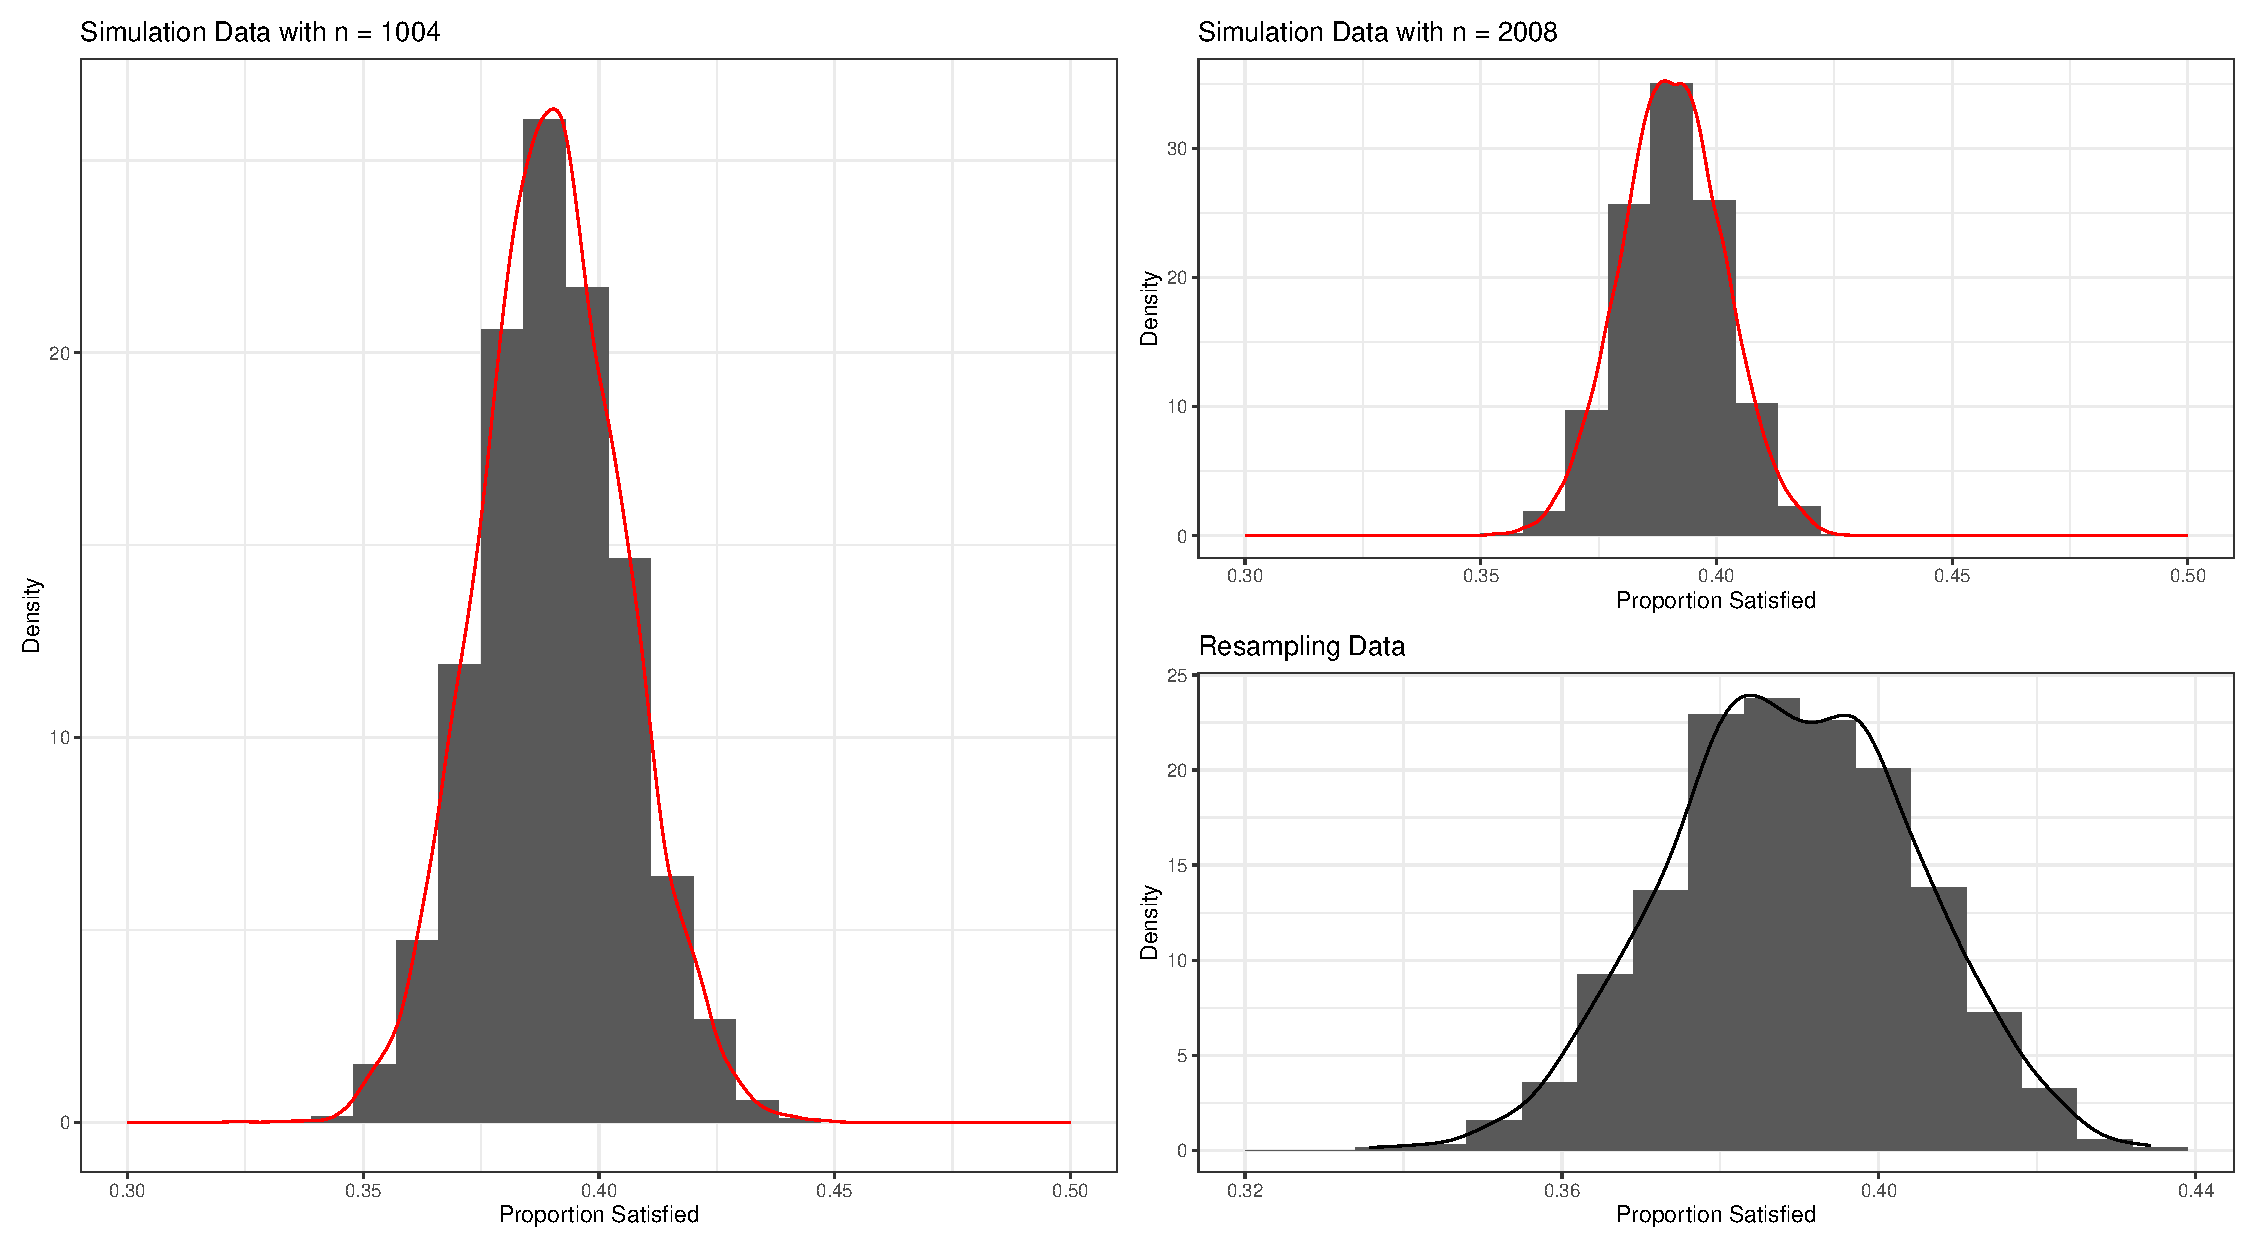
\includegraphics[scale=0.35]{graphs.pdf}
       \caption{}
     \label{moe}
     \end{center}
   \end{figure}
   \begin{figure}[H]
    \begin{center}
       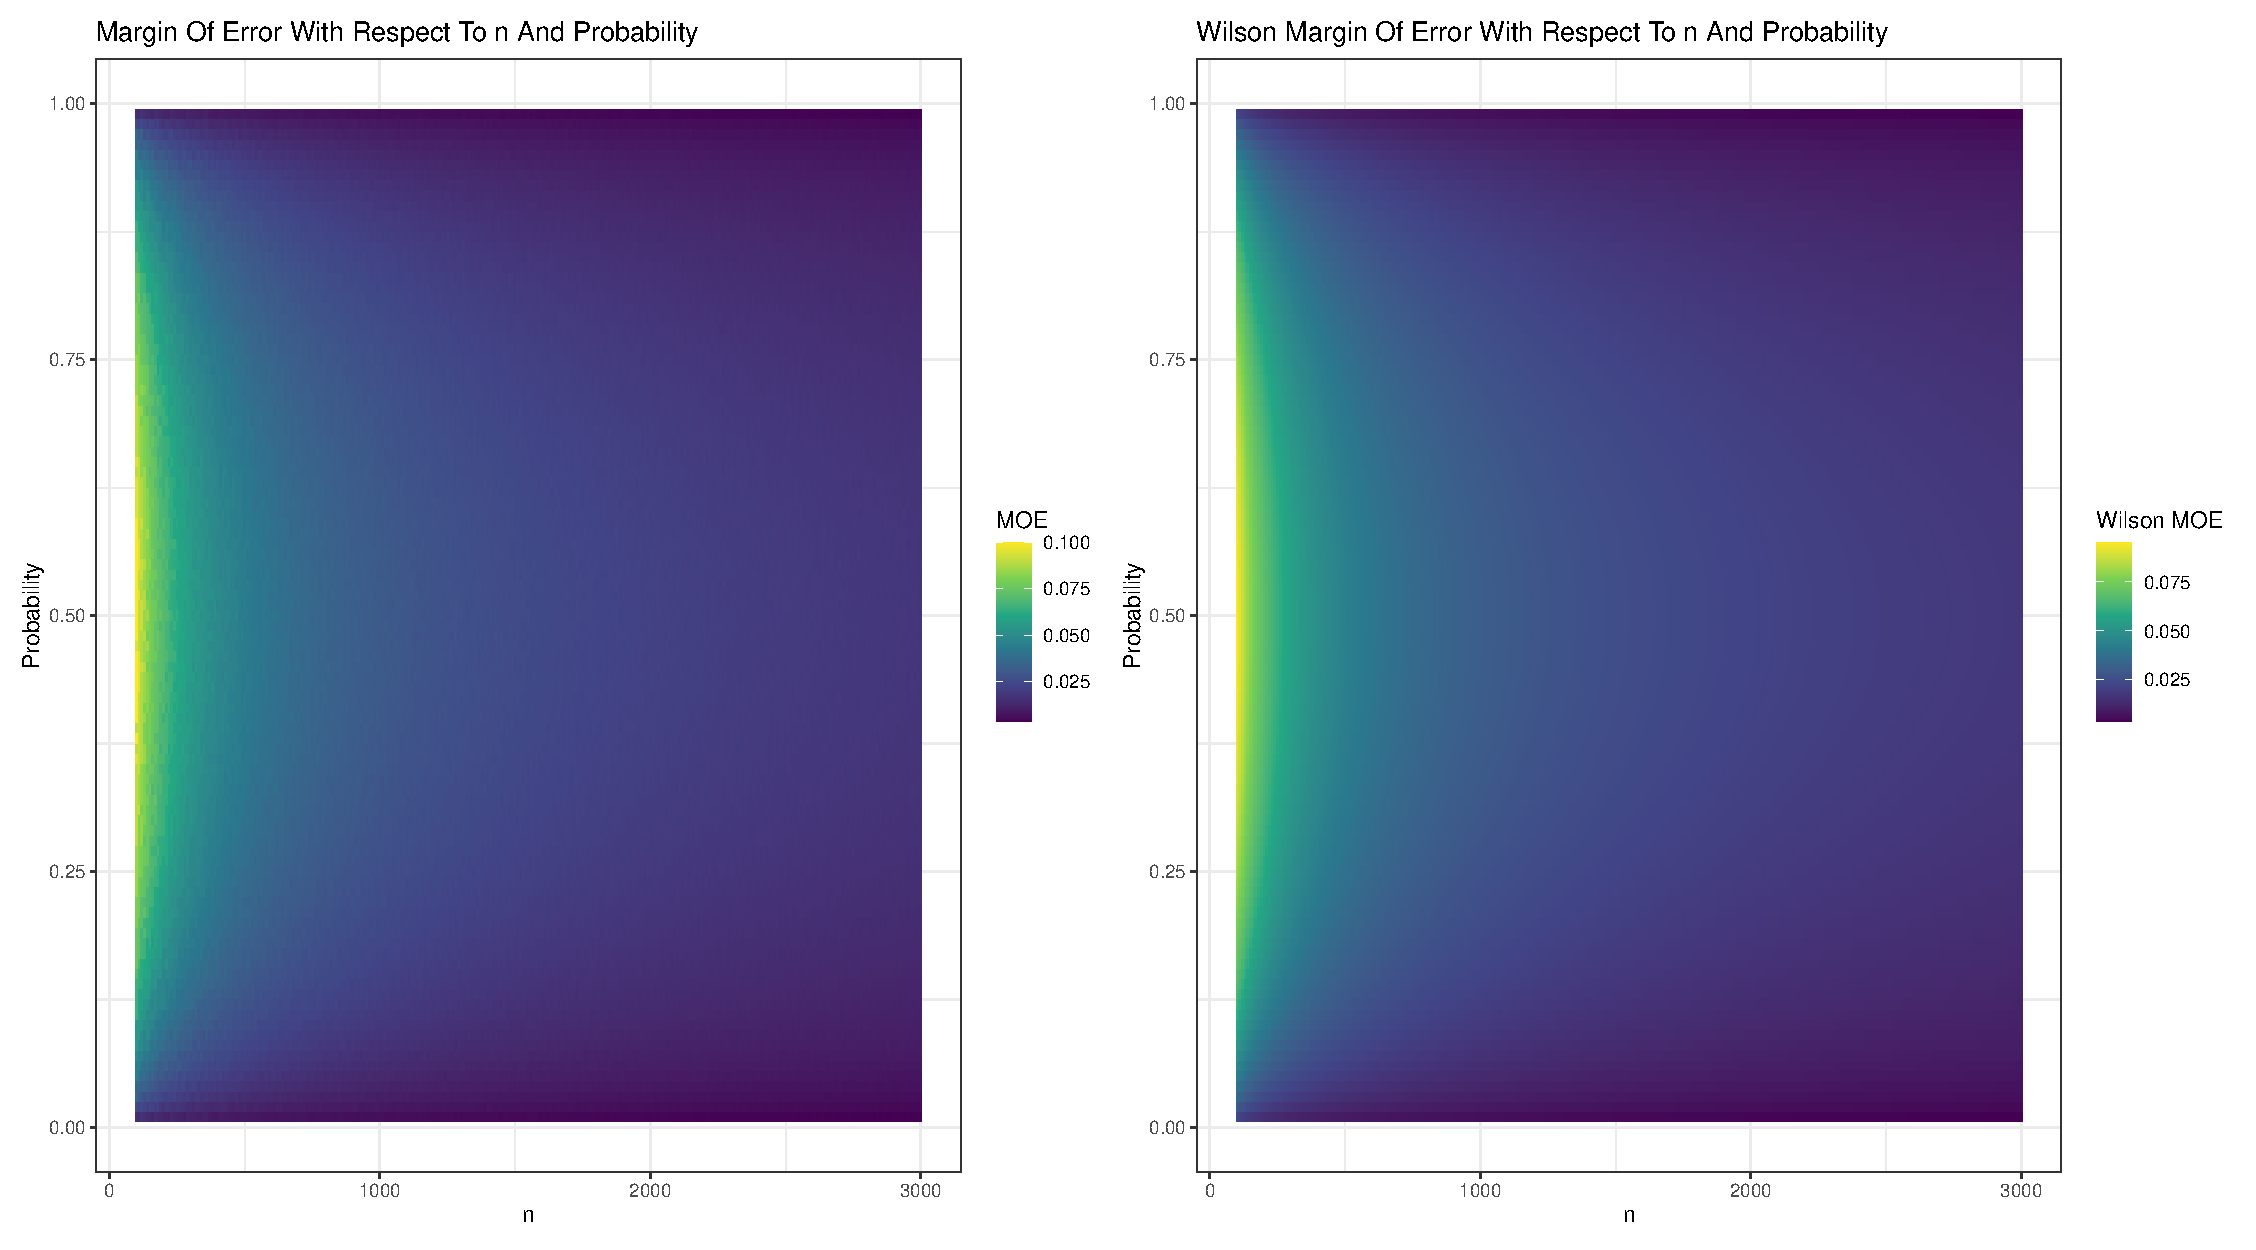
\includegraphics[scale=0.35]{raster.pdf}
       \caption{}
     \label{moe}
     \end{center}
   \end{figure}
If you have anything extra, you can add it here in the appendix. This can include images or tables that don't work well in the two-page setup, code snippets you might want to share, etc.

\end{document}
